\section{Task 4.1}
\subsection{Dataset Preparation}
This task of the project has been carried out in the following way: two CNNs were modeled, one for classifying all 4 emotions, one for only two emotions (fear and disgust).\\
In order to do so two subsets of the initial dataset were chosen: since random selection of images gave poor performance in terms of accuracy, \textbf{250 images per class were hand selected} for both CNN. The hand selection permitted to share a specific characteristic between images of the same classing (like smiling in case of happiness or eyes open widely in case of fear)\\
Since the training set obtained (80\% of the whole set of images for both cases) were not so high, \textbf{data augmentation was performed} by reflecting, slightly rotating and translating images in the following way:   

\begin{lstlisting}[language=Matlab]
%Method for image augmentation
imageAugmenter = imageDataAugmenter('RandRotation',[-20,20],...
'RandXReflection', true, ...
'RandXTranslation', [-10 10], ...
'RandYTranslation', [-10 10]);
\end{lstlisting}

In general both CNN were developed in order to obtain the best validation accuracy and minimizing at the same time the size of both CNN. A thing noticed through some experiments was that leakyReluLayers in combination with \verb|sgdm| algorithm permitted to achieve a speed up of the training process. Going deeper with the layers, Convolutional Layers decreases the stride and the filter dimension, while increasing the number of those was. MaxPooling Layers do the same thing for the stride parameter. \\
The final architectures of CNNs obtained taking into account all the points expressed were the following:

\begin{lstlisting}[language=Matlab] 
	%CNN layers for two-classes classification
	leaky_layers_two = [
		imageInputLayer(size(base_img))
		
		convolution2dLayer(16,6,'Stride',4,'Padding','same')
		batchNormalizationLayer
		leakyReluLayer
		
		maxPooling2dLayer(2,'Stride',2)
		
		convolution2dLayer(8,12,'Stride',2,'Padding','same')
		batchNormalizationLayer
		leakyReluLayer
		
		maxPooling2dLayer(2,'Stride',2)
		
		fullyConnectedLayer(40)
		fullyConnectedLayer(2)
		
		softmaxLayer
		
		classificationLayer
	];
\end{lstlisting} 

\begin{lstlisting}[language=Matlab] 
	%CNN layers for four-classes classification 
	leaky_layers_four = [
		imageInputLayer(size(base_img))
		
		convolution2dLayer(16,8,'Stride',4,'Padding','same')
		batchNormalizationLayer
		leakyReluLayer
		
		maxPooling2dLayer(2,'Stride',2)
		
		convolution2dLayer(8,16,'Stride',2,'Padding','same')
		batchNormalizationLayer
		leakyReluLayer
		
		maxPooling2dLayer(2,'Stride', 1)
		
		convolution2dLayer(4,32,'Stride',2,'Padding','same')
		batchNormalizationLayer
		leakyReluLayer
		
		maxPooling2dLayer(2,'Stride',1)
		
		fullyConnectedLayer(100)
		fullyConnectedLayer(100)
		fullyConnectedLayer(4)
		
		softmaxLayer
		
		classificationLayer
	];
\end{lstlisting} 

In the following are presented the result of training process for both CNNs:
\begin{figure}[H]
	\centering
	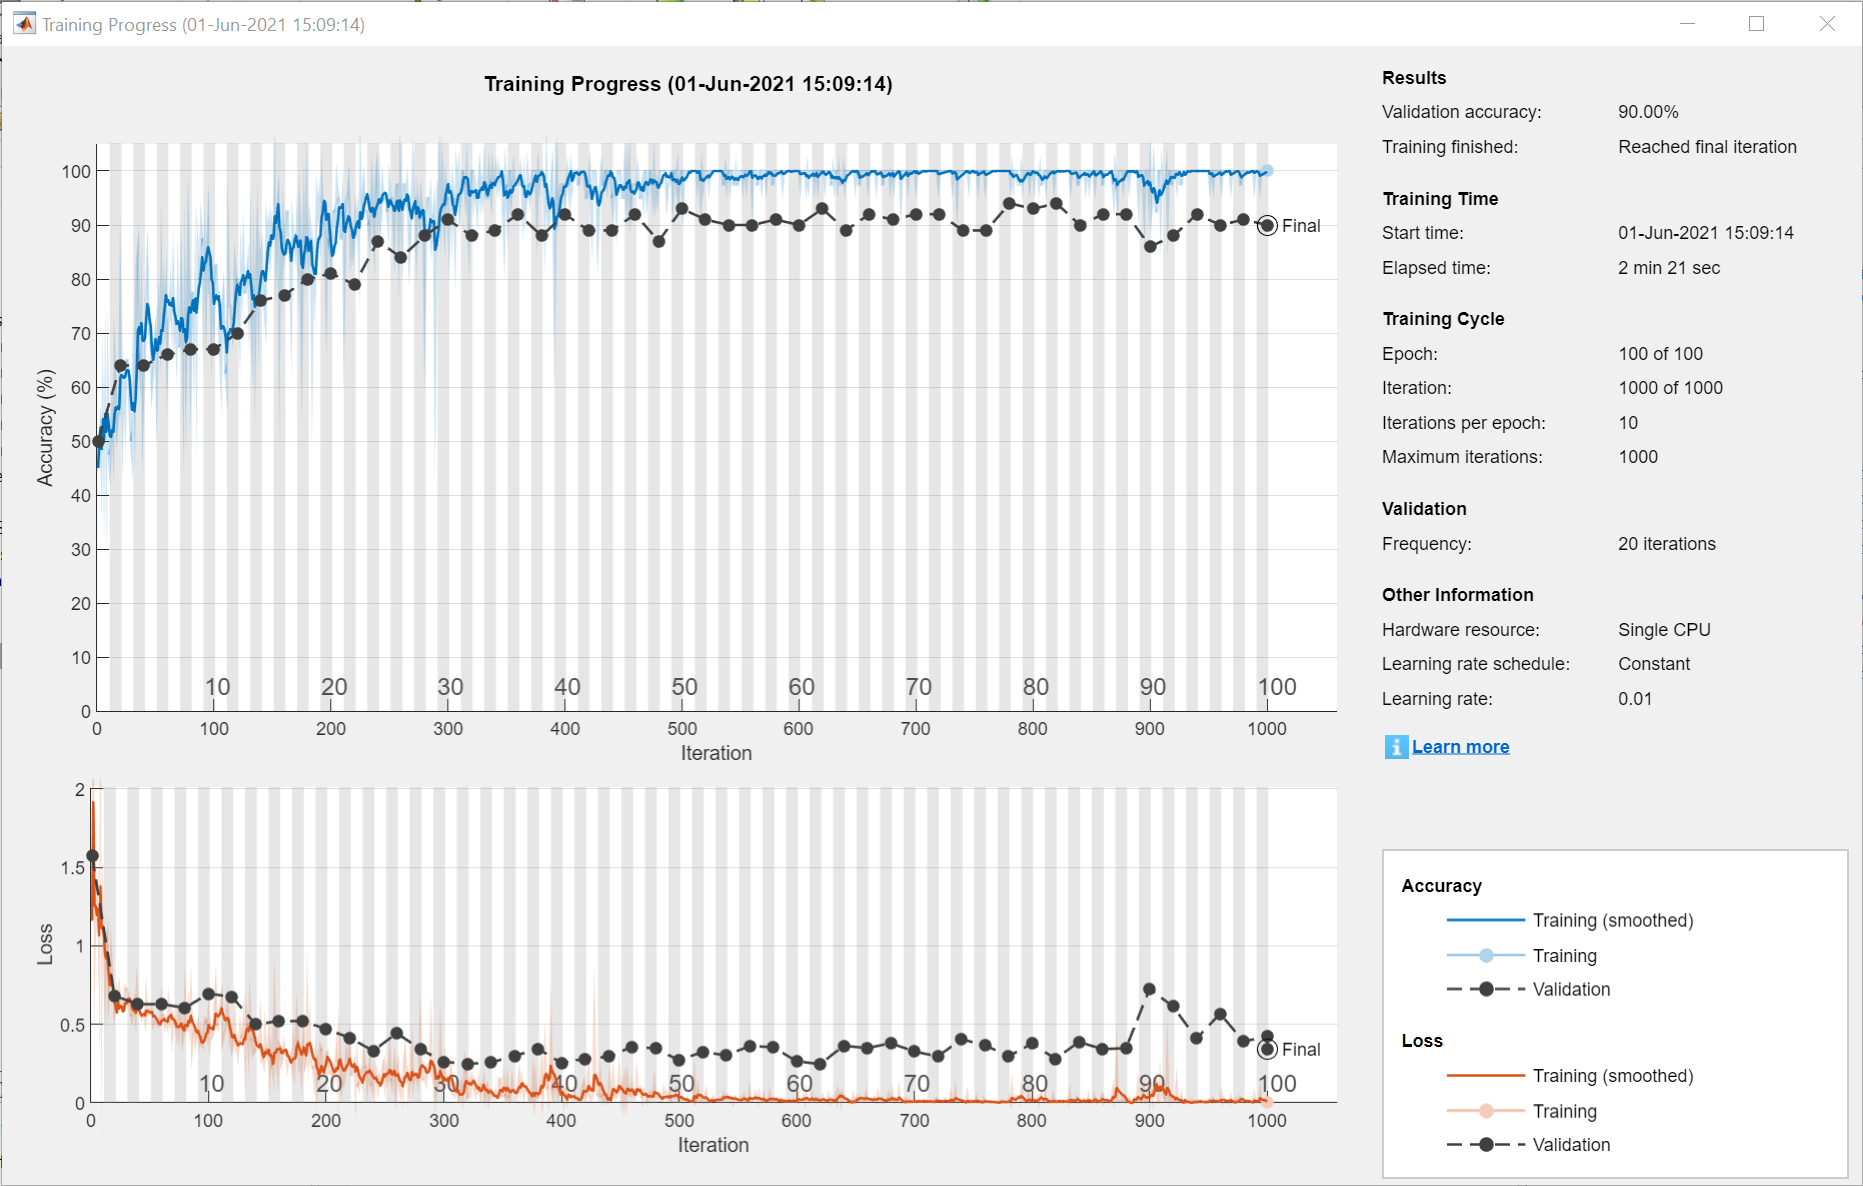
\includegraphics[width=\linewidth]{img/digust_x_fear_training.png}
	\caption{Training process of the CNN with 2 classes (disgust and fear)}
\end{figure}

\begin{figure}[H]
	\centering
	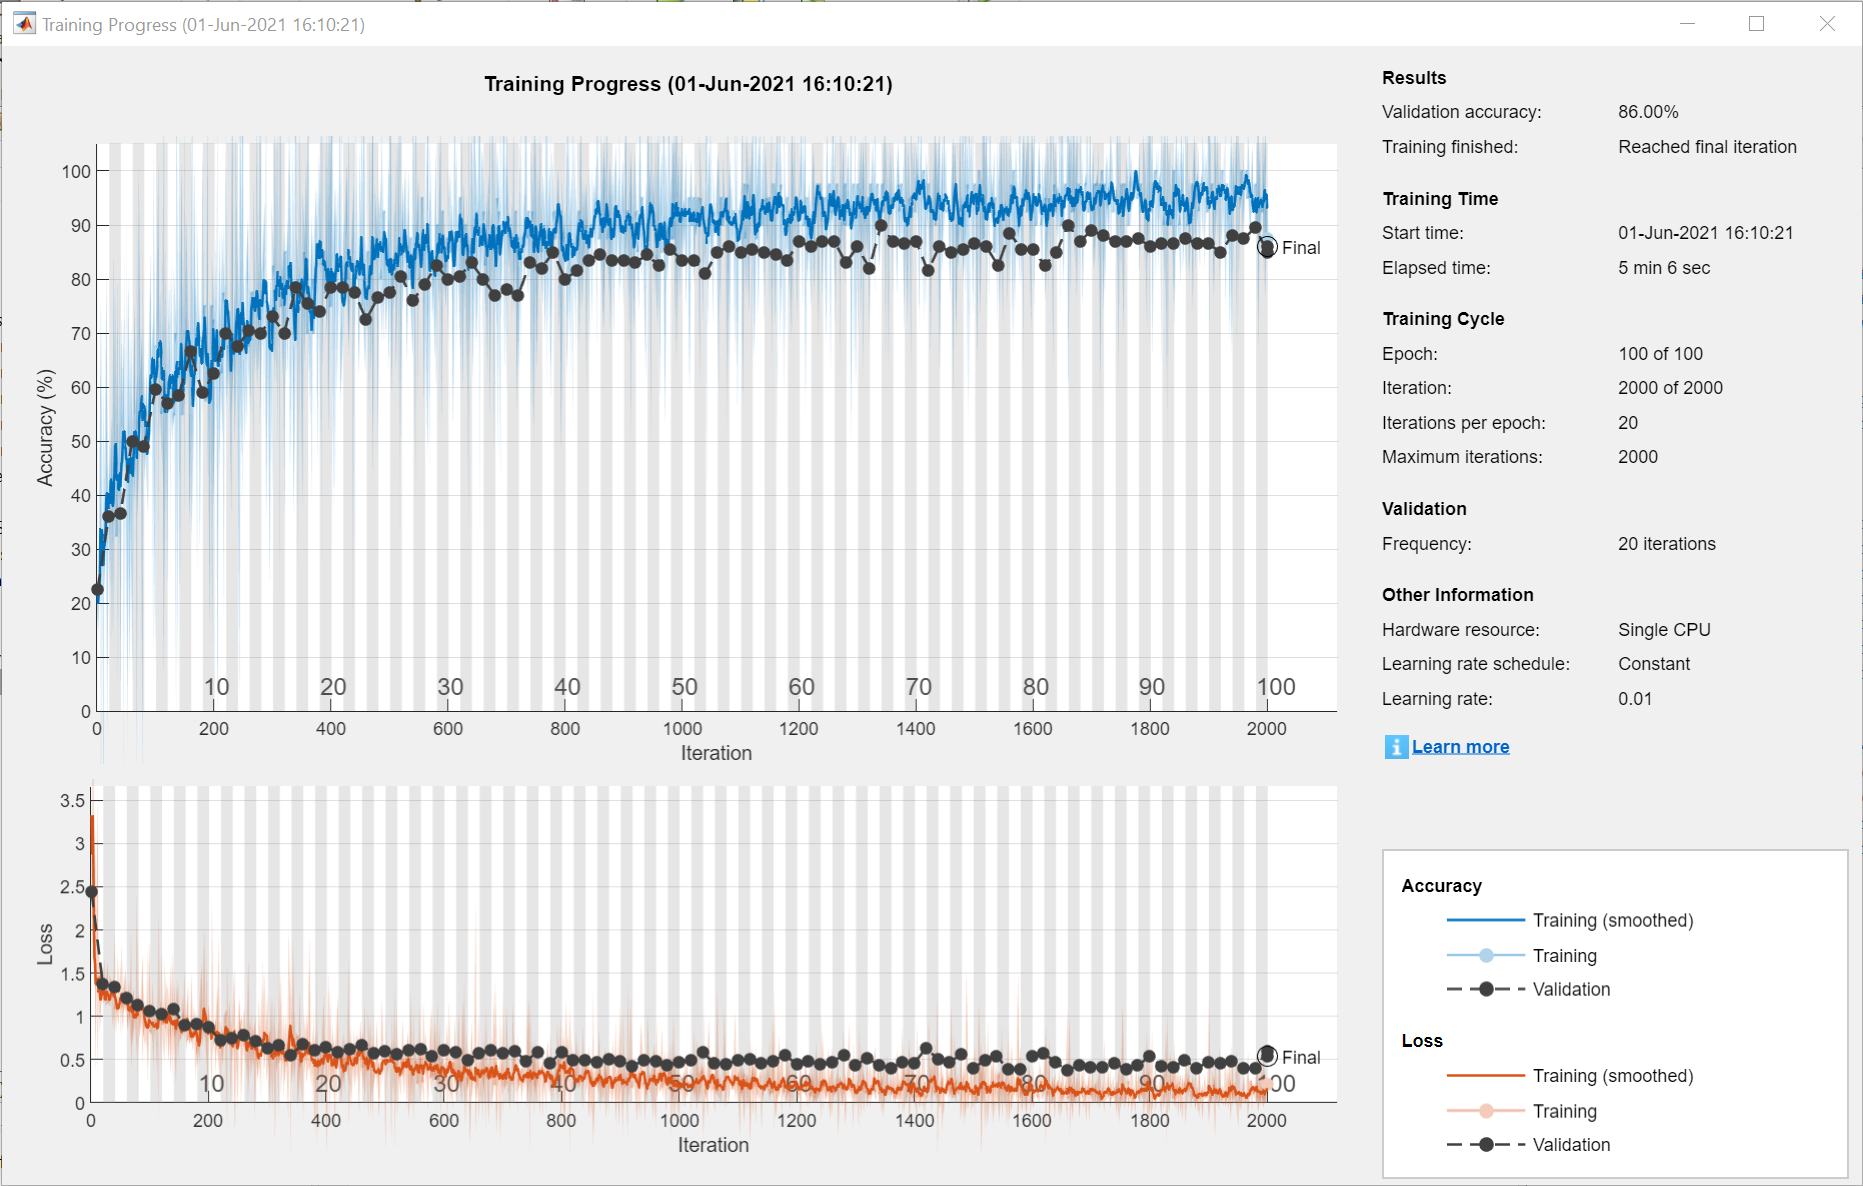
\includegraphics[width=\linewidth]{img/cnn4_training.png}
	\caption{Training process of the CNN with 4 classes}
\end{figure}

As a last point the validation accuracy was analysed in a deeper by plotting the Confusion matrix for both CNNs. In fact, during the experimentation. by modifying the hand selected images of poor classified classes, the CNNs accuracy improved. The final confusion matrix obtained are the following:  
\begin{figure}[H]
	\centering
	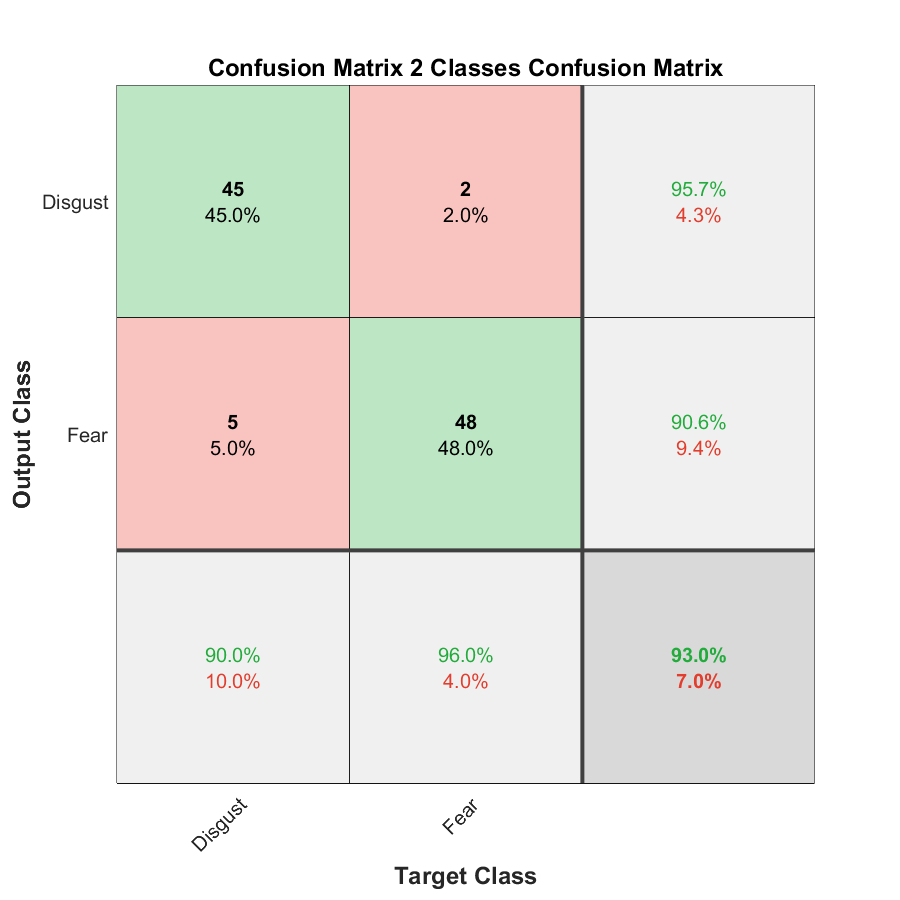
\includegraphics[width=0.6\linewidth]{img/digust_x_fear_confusion_matrix.png}
	\caption{Confusion Matrix of CNN with two classes (confusion and fear)}
\end{figure}

\begin{figure}[H]
	\centering
	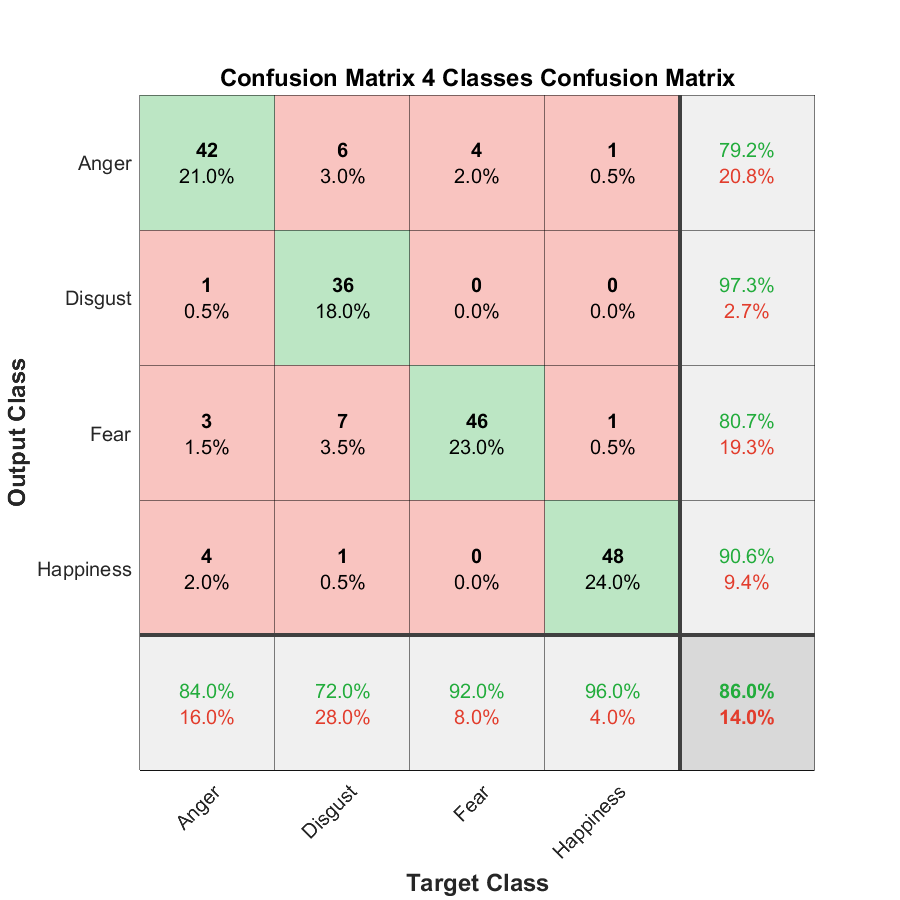
\includegraphics[width=0.7\linewidth]{img/cnn4_confusion_matrix.png}
	\caption{Confusion Matrix of CNN with four classes}
\end{figure}